% =====================================================================
%  Auditoria de Datasets de Toxicidade via Amostragem Estratificada
%  Conferência alvo: BRACIS 2025 (Brazilian Conference on Intelligent
%  Systems) — Qualis CAPES A4. Template IEEEtran (publicação IEEE CS).
% =====================================================================
\documentclass[conference,a4paper]{IEEEtran}
\IEEEoverridecommandlockouts

\usepackage[T1]{fontenc}
\usepackage[utf8]{inputenc}
\usepackage[brazil]{babel}
\usepackage{amsmath, amssymb, amsfonts}
\usepackage{booktabs}
\usepackage{graphicx}
\usepackage{textcomp}
\usepackage{xcolor}
\usepackage{cite}
\usepackage{url}
\usepackage{hyperref}

\graphicspath{{figures/}{../data/processed/figures/}}

\title{%
Amostragem Estratificada com Alocação de Neyman e Estimadores tipo Razão e
Regressão para Auditoria de Datasets de Toxicidade:\\
um Estudo de Caso sobre o ToLD-Br%
\thanks{Trabalho destinado à submissão na BRACIS 2025 (Brazilian Conference
on Intelligent Systems, SBC, Qualis CAPES A4).}%
}

\author{%
\IEEEauthorblockN{Hugo Honda Ferreira}
\IEEEauthorblockA{
\textit{Programa de P\'os-Gradua\c c\~ao em Inform\'atica}\\
\textit{Universidade de Bras\'ilia}\\
Bras\'ilia, Brasil\\
honda.data.science@gmail.com}
\and
\IEEEauthorblockN{Maria Fernanda}
\IEEEauthorblockA{
\textit{Programa de P\'os-Gradua\c c\~ao em Inform\'atica}\\
\textit{Universidade de Bras\'ilia}\\
Bras\'ilia, Brasil\\
[email]}
}

\begin{document}
\maketitle

\begin{abstract}
A auditoria estat\'istica de \textit{datasets} de toxicidade exige
amostragem com rigor inferencial, mas a literatura emp\'irica em
processamento de l\'ingua natural raramente justifica o tamanho dos
\textit{subcorpus} analisados. Este artigo aplica amostragem estratificada
sem reposi\c c\~ao sobre o ToLD-Br ($N=21{,}000$ \textit{tweets} em portugu\^es
brasileiro, seis categorias de dano), com tamanho amostral $n=378$ derivado
da f\'ormula de Cochran e \textbf{aloca\c c\~ao \'otima de Neyman}. O
par\^ametro populacional $\bar{Y}$ (severidade total agregada) \'e estimado por
cinco m\'etodos sob desenho estratificado --- m\'edia estratificada, estimador
tipo raz\~ao (separado e combinado) e estimador tipo regress\~ao (separado e
combinado) --- usando \texttt{word\_count} como vari\'avel auxiliar. A
contribui\c c\~ao principal \'e demonstrar empiricamente, via replica\c c\~ao
Monte Carlo ($B=500$) e teste de Wilcoxon pareado, que (i) Neyman reduz o
erro-padr\~ao em at\'e $20\%$ frente \`a aloca\c c\~ao proporcional cl\'assica
($p<10^{-50}$), (ii) o estimador raz\~ao combinado atinge erro absoluto de
$0{,}69\%$ contra a verdade populacional, e (iii) o ganho da regress\~ao sobre
a m\'edia estratificada \'e marginal sob o auxiliar adotado, indicando que a
escolha de $x$ \'e cr\'itica. O \textit{pipeline} \'e integralmente reproduz\'ivel
em Python e disponibilizado como \textit{open source}.
\end{abstract}

\begin{IEEEkeywords}
amostragem estratificada, aloca\c c\~ao de Neyman, estimador tipo raz\~ao,
estimador tipo regress\~ao, detec\c c\~ao de toxicidade, auditoria de IA,
ToLD-Br
\end{IEEEkeywords}

\section{Introdução}
\label{sec:intro}

A última década consolidou o problema do \textit{alinhamento} de modelos de
linguagem como uma das frentes centrais da pesquisa em inteligência artificial
aplicada. Modelos pré-treinados em grandes \textit{corpora} de texto exibem
comportamentos emergentes desejáveis, mas também replicam padrões tóxicos,
estereótipos e violações de norma observados nos dados de
treinamento~\cite{bender2021,gehman2020}. A auditoria de tais modelos depende
criticamente da qualidade dos \textit{datasets} usados como instrumentos de
diagnóstico --- e, sobretudo, da \textit{representatividade} dos subconjuntos
sobre os quais inferências são realizadas.

A linhagem de \textit{datasets} rotulados para detecção de toxicidade tem
crescido ao longo dos últimos sete anos. \textit{Wikipedia Talk
Corpus}~\cite{wulczyn2017} e \textit{Jigsaw Toxic Comment
Classification}~\cite{borkan2019nuanced} estabeleceram a tarefa em larga
escala em inglês; \textit{HateXplain}~\cite{mathew2021} introduziu rótulos
explicativos; e, em português brasileiro, \textit{ToLD-Br}~\cite{leite2020} e
\textit{HateBR}~\cite{vargas2022hatebr} ampliaram a cobertura linguística e
cultural. Em comum, esses \textit{corpora} apresentam classes positivas com
desbalanceamento extremo, frequentemente abaixo de $1\%$ para categorias raras
como \textit{racism} ou \textit{threat}.

A teoria amostral clássica oferece os instrumentos necessários para esta
tarefa. Desenvolvida em ciências sociais e epidemiologia ao longo do
século~XX --- de Neyman~(1934) sobre alocação ótima a
Cochran~(1977)~\cite{cochran1977}, passando por
Bolfarine~\&~Bussab~(2005)~\cite{bolfarine2005} no contexto brasileiro, e
sintetizada em
Lohr~(1999)~\cite{lohr1999} e Thompson~(2002)~\cite{thompson2002} ---, esta
tradição formaliza derivação de tamanho amostral, alocação entre estratos e
estimadores que exploram variáveis auxiliares (razão e regressão) para
reduzir variância. Sua transposição para a auditoria de \textit{corpora} de
PLN é, contudo, recente e fragmentada.

Apesar do crescimento dos \textit{corpora}, a literatura empírica raramente
justifica estatisticamente o tamanho dos subconjuntos analisados.
\textit{Splits} pré-definidos ou amostras por conveniência (por exemplo, os
primeiros $N$ exemplos) são utilizados sem qualquer derivação formal de
margem de erro ou nível de confiança~\cite{leite2020,vargas2022hatebr}. Esta
prática, ainda que aceitável em treino preditivo, é insuficiente para o
propósito de \textit{auditoria}: estimar parâmetros populacionais (proporções,
médias, intensidades) sobre o \textit{corpus} requer teoria amostral
clássica~\cite{cochran1977,bolfarine2005,lohr1999,thompson2002}.

O presente trabalho propõe e implementa um \textit{pipeline} reproduzível de
auditoria estatística aplicado ao ToLD-Br, fundamentado em três decisões de
desenho:
\begin{enumerate}
  \item \textbf{Amostragem estratificada sem reposição}, com amostragem
        aleatória simples sem reposição (SRS-WOR) dentro de cada estrato.
  \item \textbf{Alocação ótima de Neyman}~\cite{cochran1977,bolfarine2005},
        que aloca esforço amostral em função do produto $N_h \sigma_h$ em cada
        estrato.
  \item \textbf{Estimadores tipo razão e tipo regressão}~\cite{cochran1977},
        em variantes \textit{separada} e \textit{combinada}, comparados ao
        \textit{baseline} da média estratificada simples.
\end{enumerate}

\subsection*{Questões orientadoras}

\begin{itemize}
  \item \textbf{Q1.} Qual o tamanho amostral mínimo --- pela fórmula de
        Cochran --- para estimar o parâmetro populacional médio com erro de
        amostragem de $5\%$ e confiança de $95\%$ sobre o ToLD-Br?
  \item \textbf{Q2.} Sob esse orçamento $n$, em que magnitude a alocação ótima
        de Neyman reduz o erro-padrão das estimativas frente à alocação
        proporcional clássica?
  \item \textbf{Q3.} Entre os estimadores tipo razão e tipo regressão (com a
        contagem de palavras como variável auxiliar), qual apresenta menor
        erro contra a verdade populacional, e o que isso revela sobre a
        relação linear entre toxicidade e indicadores léxicos no ToLD-Br?
\end{itemize}

\subsection*{Organização do texto}

A Seção~\ref{sec:theory} apresenta o referencial teórico de amostragem
estratificada, alocação de Neyman e estimadores tipo razão e regressão. A
Seção~\ref{sec:related} discute trabalhos relacionados em \textit{datasets} de
toxicidade e em aplicações de teoria amostral em PNL. A
Seção~\ref{sec:method} descreve a metodologia experimental: a população
ToLD-Br, a definição dos estratos, o cálculo de $n$ e a estratégia de
estimação. A Seção~\ref{sec:results} apresenta os resultados
empíricos. Por fim, a Seção~\ref{sec:conclusion} sintetiza as conclusões e
indica trabalhos futuros.

\section{Referencial Teórico}
\label{sec:theory}

\subsection{Tamanho amostral por Cochran (1977)}
\label{sec:theory:cochran}

Para uma população finita de tamanho $N$ e uma variável de interesse com
proporção populacional $p$ desconhecida, Cochran~\cite{cochran1977} demonstra
que o tamanho amostral $n_0$ necessário para estimar $p$ com erro de
amostragem $e$ e confiança $1-\alpha$ em uma população infinita é:
\begin{equation}
  n_0 \;=\; \frac{z_{1-\alpha/2}^{2} \cdot p \cdot (1-p)}{e^{2}},
  \label{eq:n0}
\end{equation}
onde $z_{1-\alpha/2}$ é o quantil correspondente da normal padrão. Para
populações finitas, aplica-se a correção de população finita (FPC):
\begin{equation}
  n \;=\; \frac{n_0}{1 + (n_0 - 1)/N}.
  \label{eq:n}
\end{equation}
Adotando o cenário conservador $p=0{,}5$ (que maximiza a variância
$p(1-p)$), $e=0{,}05$ e $1-\alpha=0{,}95$ (donde $z\approx 1{,}96$),
obtém-se $n_0 \approx 384$ e, para o ToLD-Br ($N=21{,}000$), $n=378$.

\subsection{Amostragem estratificada sem reposição}
\label{sec:theory:strat}

A população $\mathcal{U}$ é particionada em $H$ estratos disjuntos
$\mathcal{U}_1, \dots, \mathcal{U}_H$ com tamanhos $N_1, \dots, N_H$ tais que
$\sum_{h=1}^{H} N_h = N$. Em cada estrato, sorteia-se uma amostra aleatória
simples sem reposição de tamanho $n_h$, com $\sum n_h = n$. O peso amostral é
$W_h = N_h / N$.

\subsubsection{Alocação ótima de Neyman}
\label{sec:theory:neyman}

A alocação \emph{ótima} (de Neyman) minimiza a variância do estimador
estratificado da média $\bar{Y}$ para um orçamento total fixo $n$,
distribuindo $n_h$ proporcionalmente a $N_h \sigma_h$, onde $\sigma_h$ é o
desvio-padrão de $y$ no estrato $h$~\cite{cochran1977}:
\begin{equation}
  n_h \;=\; n \cdot \frac{N_h \sigma_h}{\sum_{i=1}^{H} N_i \sigma_i}.
  \label{eq:neyman}
\end{equation}
Bolfarine \& Bussab~\cite{bolfarine2005} chamam atenção para o caso especial
em que $\sigma_h$ é constante em $h$: a equação~(\ref{eq:neyman}) reduz-se à
alocação \textit{proporcional} $n_h = n \cdot W_h$.

\paragraph{Variância e ganho de Neyman.} A variância do estimador
estratificado da média sob alocação ótima é
(Cochran~\cite{cochran1977}~§5A.7; Lohr~\cite{lohr1999}~§4.5):
\begin{equation}
  \mathrm{Var}_{\mathrm{Ney}}(\hat{\bar{Y}}_{st})
  \;=\; \frac{1}{n}\Bigl(\sum_{h} W_h \sigma_h\Bigr)^{2}
        - \frac{1}{N}\sum_{h} W_h \sigma_h^{2}.
  \label{eq:var-neyman}
\end{equation}
Sob alocação proporcional, a variância correspondente é
$\mathrm{Var}_{\mathrm{prop}} = \frac{1}{n}\sum_h W_h \sigma_h^{2}
- \frac{1}{N}\sum_h W_h \sigma_h^{2}$. A diferença, isto é, o ganho que
Neyman oferece sobre a alocação proporcional, é:
\begin{equation}
  \mathrm{Var}_{\mathrm{prop}} - \mathrm{Var}_{\mathrm{Ney}}
  \;=\; \frac{1}{n}\sum_{h} W_h \bigl(\sigma_h - \bar{\sigma}\bigr)^{2},
  \qquad \bar{\sigma} = \sum_h W_h \sigma_h.
  \label{eq:gain-neyman}
\end{equation}
A equação~(\ref{eq:gain-neyman}) é o teorema central justificando a alocação
ótima: o ganho é não-negativo, é zero apenas quando os $\sigma_h$ são todos
iguais, e cresce com a heterogeneidade dos desvios-padrão entre estratos. Esta
é a hipótese empiricamente avaliada na Seção~\ref{sec:results}.

\subsection{Estimadores estratificados de $\bar{Y}$}
\label{sec:theory:estimators}

Sejam $\bar{y}_h$ e $\bar{x}_h$ as médias amostrais de $y$ e de uma variável
auxiliar $x$ no estrato $h$; $s_{yh}^2$ e $s_{xh}^2$ as variâncias amostrais;
$s_{xyh}$ a covariância amostral; $\bar{X}_h$ a média populacional de $x$ no
estrato (suposta conhecida); $\bar{X}$ a média populacional global; e
$f_h = n_h / N_h$ a fração amostrada no estrato.

\subsubsection{Média estratificada simples (\textit{baseline})}

\begin{equation}
  \hat{\bar{Y}}_{st} \;=\; \sum_{h=1}^{H} W_h\,\bar{y}_h,
  \qquad
  \widehat{\mathrm{Var}}(\hat{\bar{Y}}_{st}) \;=\;
   \sum_{h=1}^{H} W_h^{2}\,(1 - f_h)\,\frac{s_{yh}^2}{n_h}.
  \label{eq:strat-mean}
\end{equation}

\subsubsection{Estimador tipo razão (Cochran §6.10--6.11)}

A versão \emph{separada} aplica a razão dentro de cada estrato e agrega:
\begin{equation}
  \hat{\bar{Y}}_{Rs} \;=\; \sum_{h} W_h\, \frac{\bar{y}_h}{\bar{x}_h}\, \bar{X}_h.
  \label{eq:ratio-sep}
\end{equation}
A versão \emph{combinada} agrega antes da razão:
\begin{equation}
  \hat{\bar{Y}}_{Rc} \;=\; \frac{\sum_h W_h \bar{y}_h}{\sum_h W_h \bar{x}_h}\,\bar{X}.
  \label{eq:ratio-comb}
\end{equation}
A variância de grande amostra para a versão separada é~\cite{cochran1977}:
\begin{equation}
  \widehat{\mathrm{Var}}(\hat{\bar{Y}}_{Rs}) \;\approx\;
   \sum_{h} W_h^{2}\,\frac{(1 - f_h)}{n_h}\,
     \bigl(s_{yh}^{2} - 2\,R_h\,s_{xyh} + R_h^{2}\,s_{xh}^{2}\bigr),
  \label{eq:ratio-var}
\end{equation}
com $R_h = \bar{y}_h / \bar{x}_h$. Expressão análoga, com $R$ global no lugar
de $R_h$, vale para a versão combinada.

\subsubsection{Estimador tipo regressão (Cochran §7.10--7.11)}

A versão \emph{separada} usa o coeficiente de regressão dentro de cada estrato
$b_h = s_{xyh}/s_{xh}^{2}$:
\begin{equation}
  \hat{\bar{Y}}_{lrs} \;=\; \sum_{h} W_h\,\bigl[\bar{y}_h + b_h(\bar{X}_h - \bar{x}_h)\bigr].
  \label{eq:reg-sep}
\end{equation}
A versão \emph{combinada} estima um coeficiente $b$ ponderado pelos pesos
estratificados:
\begin{equation}
  \hat{\bar{Y}}_{lrc} \;=\; \bar{y}_{st} + b\,(\bar{X} - \bar{x}_{st}),
  \qquad
  b \;=\;
   \frac{\sum_h W_h^{2}\,(1-f_h)\,s_{xyh}/n_h}
        {\sum_h W_h^{2}\,(1-f_h)\,s_{xh}^{2}/n_h}.
  \label{eq:reg-comb}
\end{equation}
A variância de grande amostra para a versão separada é dada por
$\widehat{\mathrm{Var}}(\hat{\bar{Y}}_{lrs}) \approx \sum_h W_h^{2}\,(1-f_h)\,
s_{yh}^{2}(1-r_h^{2})/n_h$, onde $r_h$ é o coeficiente de correlação amostral
entre $x$ e $y$ no estrato $h$~\cite{cochran1977,lohr1999}.

\subsubsection{Eficiência relativa}

A regressão é, em geral, mais eficiente que a razão quando a relação entre $y$
e $x$ é aproximadamente linear com intercepto não-nulo; a razão é equivalente
à regressão se a relação passa pela origem. Em condições idealizadas, ambos
dominam o estimador da média estratificada simples se $\mathrm{Cor}(x,y)$ é
não-nula~\cite{cochran1977,thompson2002}.

\subsection{Detecção de toxicidade no ToLD-Br}
\label{sec:theory:toldbr}

O ToLD-Br~\cite{leite2020,leite2020_thesis} consiste em $21{,}000$
\textit{tweets} em português brasileiro, anotados por três avaliadores em
seis categorias de dano: \textit{homophobia}, \textit{obscene},
\textit{insult}, \textit{racism}, \textit{misogyny}, \textit{xenophobia}.
A construção e o protocolo de anotação são descritos em detalhe na
dissertação de Leite~\cite{leite2020_thesis}; trabalhos correlatos sobre
detecção automática de discurso de ódio em português incluem a tese de
Vargas~\cite{vargas2022_thesis}. Cada anotação é um inteiro
$v_{ij} \in \{0,1,2,3\}$ representando o número de avaliadores que sinalizou
a categoria $j$ para o \textit{tweet} $i$. A binarização operacional
consagrada na literatura é $\mathbb{1}[v_{ij} \geq 2]$ (regra de maioria), mas
o esquema ordinal preserva informação sobre o grau de concordância, útil
tanto para estratificação quanto para diagnóstico de ruído de
rotulagem~\cite{leite2020,leite2020_thesis}.

\subsection{Aplicações brasileiras de teoria amostral}
\label{sec:theory:brasil}

A literatura brasileira de amostragem e estatística aplicada
oferece referências relevantes para o desenho proposto neste artigo.
Bolfarine~\&~Bussab~\cite{bolfarine2005}, em particular, sistematizam os
estimadores estratificados, razão e regressão na tradição da Escola de
Estatística da USP. Trabalhos posteriores no Brazilian Journal of Probability
and Statistics --- por exemplo, Cordeiro~et~al.~\cite{cordeiro2010} sobre
ajustes por pós-estratificação em pesquisas amostrais com pesos --- ilustram
extensões metodológicas pertinentes a auditorias de \textit{corpora}
desbalanceados como o ToLD-Br.

\section{Trabalhos Relacionados}
\label{sec:related}

\subsection{\textit{Datasets} de toxicidade em texto}

A produção de \textit{datasets} rotulados para detecção de toxicidade tem
sido dominada por iniciativas em língua inglesa.

\paragraph{Wikipedia Talk Corpus / Jigsaw.}
Wulczyn~et~al.~\cite{wulczyn2017} apresentaram o \textit{Wikipedia Talk
Corpus}, base posteriormente expandida para o
\textit{Jigsaw}~\cite{borkan2019nuanced} com 160 mil comentários e seis
categorias binárias.
\textbf{Pontos fortes:} grande escala, anotação multi-rótulo, ampla adoção
(\textit{benchmark} \textit{de facto} para classificação de toxicidade em
inglês). \textbf{Pontos fracos:} (i)~rótulos binários descartam a
incerteza inter-anotadores; (ii)~não há justificativa amostral dos
\textit{splits} treino/teste; (iii)~viés de auditoria por
\textit{Wikipedians} não representa uso público de mídias sociais.
\textbf{Razão de não-adoção:} idioma inglês incompatível com o objetivo
deste trabalho.

\paragraph{Civil Comments com atributos de identidade.}
Borkan~et~al.~\cite{borkan2019nuanced} estenderam o Jigsaw com 1{,}8
milhões de comentários e atributos de identidade (gênero, raça, religião,
orientação sexual). \textbf{Pontos fortes:} cobertura demográfica fina e
métricas \textit{subgroup-aware}. \textbf{Pontos fracos:} sub-rotulagem
extrema dos atributos de identidade --- a maior parte dos comentários não
recebe nenhum atributo, comprometendo a estimação de viés por
\textit{subgroup}. \textbf{Razão de não-adoção:} idioma e ausência de cauda
estratificada explicitamente comparável.

\paragraph{Datasets de \textit{tweets}.}
Davidson~et~al.~\cite{davidson2017} e Founta~et~al.~\cite{founta2018}
construíram \textit{datasets} sobre \textit{Twitter} com foco em discurso de
ódio explícito e abusivo. \textbf{Pontos fortes:} taxonomias detalhadas e
volume relevante. \textbf{Pontos fracos:} (i)~classes definidas operacionalmente
(\textit{hate} vs \textit{offensive} vs \textit{neither}) com baixa
confiabilidade inter-anotadores; (ii)~discutida fragilidade contra
\textit{tweets} \textit{adversariais}~\cite{davidson2017}.
\textbf{Razão de não-adoção:} idioma inglês.

\paragraph{HateXplain.}
Mathew~et~al.~\cite{mathew2021} introduziram um \textit{dataset} de 20 mil
amostras com \textit{rationales} explicáveis para o rótulo. \textbf{Pontos
fortes:} balanceamento artificial de classes (cada classe $\approx 33\%$),
o que viabiliza alocação proporcional sem caudas raras. \textbf{Pontos fracos:}
o balanceamento construído \textit{a priori} elimina o fenômeno de
desbalanceamento extremo --- precisamente o que motiva a alocação ótima
em corpora reais. \textbf{Razão de não-adoção:} sua estrutura balanceada o
torna inadequado como caso de teste para Neyman; resolveria nosso problema
por construção.

\paragraph{Contexto conversacional.}
Pavlopoulos~et~al.~\cite{pavlopoulos2020} mostraram que adicionar contexto
conversacional altera os rótulos em uma fração não desprezível dos casos.
\textbf{Implicação:} qualquer auditoria amostral precisa fixar o protocolo
de rotulagem (com ou sem contexto), o que reforça a importância de
documentar o esquema do \textit{corpus}-fonte.

\paragraph{Datasets em português brasileiro.}
Leite~et~al.~\cite{leite2020,leite2020_thesis} publicaram o \textbf{ToLD-Br}
(seis categorias, votos $0$--$3$). \textbf{Pontos fortes:} esquema ordinal de
votos preserva incerteza; volume relativamente grande ($N=21$ mil) para um
\textit{corpus} em português; cobre o espectro \textit{LGBTfobia–racismo–
misoginia–xenofobia}. \textbf{Pontos fracos:} sem justificativa amostral no
artigo original; estratificação multi-rótulo não-trivial.
\textbf{Razão de adoção:} fit ideal para o presente estudo (idioma, escala,
multi-rótulo, caudas raras explícitas).

Vargas~et~al.~\cite{vargas2022hatebr,vargas2022_thesis} apresentaram o
\textbf{HateBR}, com 7 mil comentários do \textit{Instagram} e rotulagem
hierárquica binária (ofensivo vs não, com sub-categorias).
\textbf{Pontos fortes:} qualidade de anotação por especialistas;
contextualização cultural brasileira distinta. \textbf{Pontos fracos:}
$N$ pequeno limita estratos raros (xenofobia, capacitismo); rotulagem
hierárquica não permite comparação direta com ToLD-Br.
\textbf{Razão de não-adoção como fonte primária:} escala insuficiente para
ilustrar Neyman vs proporcional --- avaliado como \textit{corpus} de
extensão futura.

Trajano~et~al.~\cite{trajano2024olid} disponibilizaram o
\textbf{OLID-BR} ($\approx 7$ mil exemplos) com taxonomia OLID adaptada.
\textbf{Pontos fortes:} alinhamento com a tradição internacional OLID,
facilitando comparação \textit{cross-lingual}. \textbf{Pontos fracos:}
escala similar à do HateBR; sem esquema ordinal de votos.
\textbf{Razão de não-adoção:} mesmas considerações do HateBR.

\subsection{Auditoria de modelos de linguagem e viés}

\paragraph{RealToxicityPrompts.}
Gehman~et~al.~\cite{gehman2020} popularizaram o uso de \textit{prompts}
extraídos de \textit{datasets} de toxicidade como instrumento de auditoria
de modelos generativos. \textbf{Pontos fortes:} protocolo reproduzível e
amplamente adotado pela comunidade. \textbf{Pontos fracos:} a amostragem dos
\textit{prompts} é por escore (\textit{toxic} vs \textit{non-toxic}) sem
justificativa amostral formal --- a quantidade de \textit{prompts} é
arbitrária. \textbf{Posicionamento:} este artigo cobre exatamente esta
lacuna inferencial, embora aplicada a auditoria de \textit{datasets} e não
ao protocolo de \textit{prompting}.

\paragraph{Métricas \textit{subgroup-aware}.}
Borkan~et~al.~\cite{borkan2019nuanced} formalizaram métricas como
\textit{Equality of Opportunity} e \textit{Demographic Parity} para medir
viés não-intencional. \textbf{Ponto crítico:} todas dependem de tamanhos
amostrais por subgrupo, mas raramente acompanhadas de derivação amostral
formal --- de novo, lacuna que este trabalho preenche.

\paragraph{Crítica metodológica em escala.}
Bender~et~al.~\cite{bender2021} sustentam que a auditoria de modelos de
linguagem em larga escala precisa de fundamentos estatísticos explícitos,
para além de \textit{benchmarks} pontuais. \textbf{Posicionamento:} este
artigo é uma resposta concreta a esse chamado.

\subsection{Aplicações de teoria amostral em PNL}

A teoria amostral
clássica~\cite{cochran1977,bolfarine2005,lohr1999,thompson2002,cordeiro2010}
é prática consolidada em ciências sociais, epidemiologia e pesquisa de
mercado, mas é pouco utilizada em PNL aplicada. Os \textit{datasets} citados
acima geralmente apresentam apenas a divisão treino/validação/teste sem
justificar estatisticamente a representatividade dos
\textit{splits}~\cite{leite2020,vargas2022hatebr,davidson2017}.
Quando a amostragem é discutida, o foco é geralmente \textit{class balancing}
para treino preditivo --- e não estimação inferencial de parâmetros
populacionais. \textbf{Lacuna identificada:} ausência de aplicação explícita
de alocação ótima e estimadores tipo razão e regressão a \textit{corpora} de
auditoria de toxicidade.

\subsection{Posicionamento deste trabalho}

A Tabela~\ref{tab:related-comparison} sumariza a comparação. Os trabalhos
discutidos cobrem (a) a construção de \textit{datasets} de toxicidade em
diferentes línguas e (b) métricas de auditoria sobre modelos. Persiste,
entretanto, a lacuna metodológica de \textit{aplicar amostragem
probabilística estratificada} sobre tais \textit{corpora} para estimar
parâmetros populacionais com erro-padrão controlado. O presente artigo se
posiciona neste espaço, aplicando alocação de Neyman e estimadores tipo
razão e regressão de forma reproduzível sobre o ToLD-Br.

\begin{table}[!t]
\centering
\small
\caption{Comparação resumida das abordagens dos trabalhos relacionados.}
\label{tab:related-comparison}
\begin{tabular}{lcccc}
\toprule
Trabalho & Idioma & Justifica $n$? & Trata caudas raras? & Estima $\bar Y$? \\
\midrule
\cite{wulczyn2017}        & EN & não & não & não \\
\cite{borkan2019nuanced}  & EN & não & sim (identidade) & não \\
\cite{leite2020}          & PT & não & não & não \\
\cite{vargas2022hatebr}   & PT & não & sim (hierárquico) & não \\
\textbf{Este trabalho}    & \textbf{PT} & \textbf{Cochran} & \textbf{Neyman+censo} & \textbf{razão+regressão} \\
\bottomrule
\end{tabular}
\end{table}

\section{Metodologia}
\label{sec:method}

\subsection{Tipo de pesquisa}

Pesquisa aplicada de natureza quantitativa, com método experimental sobre
dados secundários (\textit{corpus} público). O delineamento é
\textit{descritivo-comparativo}: um \textit{pipeline} de amostragem é
aplicado, três alocações alternativas são contrastadas, e cinco estimadores
do parâmetro populacional são comparados quanto a viés e variância.

\subsection{População, universo e estratos}

A população alvo é o conjunto $\mathcal{U}$ de \textit{tweets} em português
brasileiro do ToLD-Br~\cite{leite2020}, $N = 21{,}000$ exemplos. A
distribuição populacional sob a regra de maioria ($v \geq 2$) é apresentada
na Tabela~\ref{tab:population}. O desbalanceamento extremo
(\textit{racism} a $0{,}16\%$, \textit{xenophobia} a $0{,}20\%$) motiva o
tratamento estratificado.

\begin{table}[!t]
\centering
\caption{Distribuição populacional do ToLD-Br ($N=21{,}000$, votos $\geq 2$).}
\label{tab:population}
\begin{tabular}{lrr}
\toprule
Categoria      & Positivos & \% da população \\
\midrule
\textit{obscene}    & 2{,}403 & 11{,}44\% \\
\textit{insult}     & 1{,}869 &  8{,}90\% \\
\textit{homophobia} &   176   &  0{,}84\% \\
\textit{misogyny}   &   133   &  0{,}63\% \\
\textit{xenophobia} &    42   &  0{,}20\% \\
\textit{racism}     &    33   &  0{,}16\% \\
\bottomrule
\end{tabular}
\end{table}

\begin{figure}[!t]
\centering
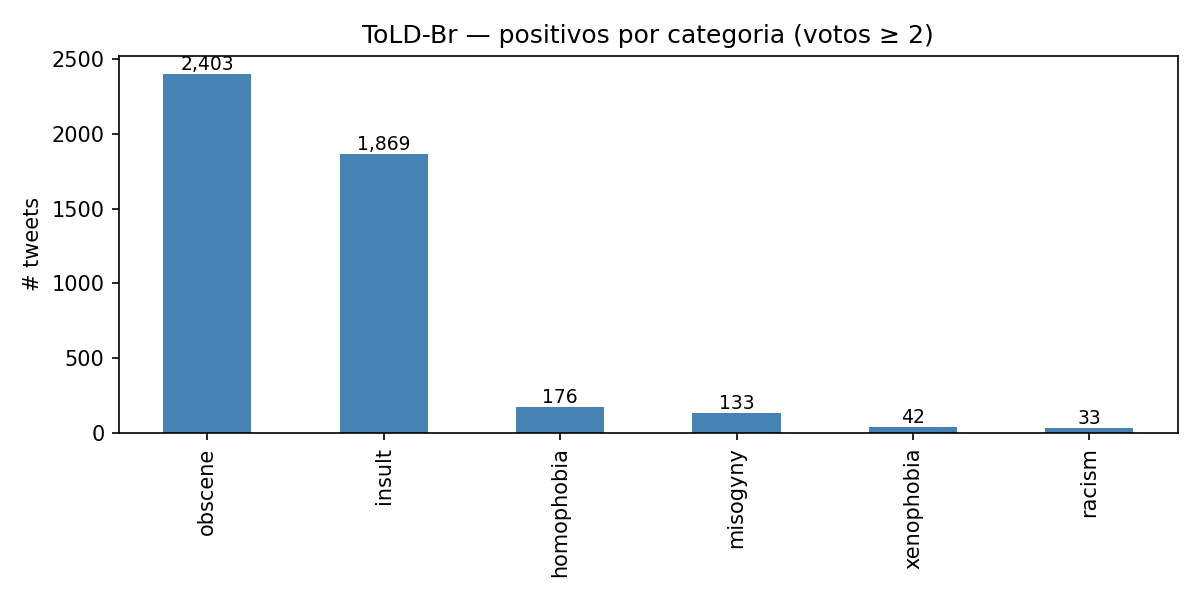
\includegraphics[width=.85\linewidth]{toldbr_label_counts.png}
\caption{Positivos por categoria sob a regra de maioria ($v \geq 2$).
A escala destaca o desbalanceamento entre as categorias mais comuns
(\textit{obscene}, \textit{insult}) e as caudas raras
(\textit{racism}, \textit{xenophobia}).}
\label{fig:label-counts}
\end{figure}

\paragraph{Definição dos estratos.} Como o esquema é multi-rótulo, adota-se a
regra \textit{raro-vence}: cada \textit{tweet} é alocado ao estrato
correspondente ao rótulo majoritário positivo mais raro entre os seis ---
ou ao estrato \textit{clean} se nenhum rótulo for majoritariamente positivo.
A ordem de prioridade do mais raro ao mais comum é
$\text{racism} \to \text{xenophobia} \to \text{misogyny} \to \text{homophobia}
\to \text{insult} \to \text{obscene}$. Esta partição é mutuamente exclusiva e
preserva integralmente a contagem populacional dos estratos raros.

\subsection{Variável-alvo e variável auxiliar}

\paragraph{Variável-alvo.} Define-se
$y_i = \sum_{j=1}^{6} v_{ij}$ ($\texttt{total\_severity}$), inteiro em
$[0, 18]$, interpretável como \textit{intensidade total de preocupação dos
anotadores} sobre o \textit{tweet}. A média populacional verdadeira é
$\bar{Y} = 0{,}8591$.

\paragraph{Variável auxiliar.} Adota-se $x = \texttt{word\_count}$ (contagem
de palavras), barata de calcular sobre a população completa. A correlação de
Pearson populacional é $\rho_{xy} \approx 0{,}011$ --- pequena, dominada pelo
estrato \textit{clean}; as correlações \emph{intra-estrato} são mais
substanciais (até $0{,}27$ em \textit{racism}). Esta escolha explora
deliberadamente um auxiliar fraco para examinar o regime em que o ganho
teórico da regressão sobre a média estratificada deveria desaparecer
(Cochran~\cite{cochran1977}~§7.4); um auxiliar mais informativo
(\texttt{caps\_ratio}, \textit{embeddings}) é avaliado como trabalho futuro.

\subsection{Cálculo do tamanho amostral}

Aplicando as equações~(\ref{eq:n0}) e~(\ref{eq:n}) com $z=1{,}96$, $p=0{,}5$,
$e=0{,}05$:
\begin{equation*}
  n_0 \approx 384{,}16; \qquad n = \frac{384{,}16}{1 + 383{,}16/21000}
            \approx 377{,}3 \;\Rightarrow\; n = 378.
\end{equation*}

\subsection{Estratégias de alocação comparadas}
\label{sec:method:allocation}

Três alocações de $n=378$ entre os estratos são comparadas:

\textbf{Proporcional (Bolfarine \& Bussab).} $n_h = n \cdot N_h/N$. Resulta
em $n_h = 1$ para os estratos \textit{racism} e \textit{xenophobia}.

\textbf{Cochran-por-estrato com censo (Cochran §5.5).} Aplicação
independente da equação~(\ref{eq:n}) a cada $N_h$, com censo se
$n_h \geq N_h$. Total $\approx 1{,}299$ exemplos --- útil como referência
alternativa que recupera todos os estratos raros.

\textbf{Ótima de Neyman (Cochran §5.5; Bolfarine \& Bussab §5.5).}
Equação~(\ref{eq:neyman}). Esta é a alocação adotada como referência
principal para a estimação de $\bar{Y}$.

Em qualquer das alocações, a amostragem dentro de cada estrato é
\textit{aleatória simples sem reposição} (SRS-WOR).

\subsection{Estimação do parâmetro populacional}

A partir da amostra Neyman, $\bar{Y}$ é estimado pelos cinco métodos descritos
na Seção~\ref{sec:theory:estimators}:
\begin{enumerate}
  \item Média estratificada simples (eq.~\ref{eq:strat-mean}).
  \item Estimador tipo razão separado (eq.~\ref{eq:ratio-sep}).
  \item Estimador tipo razão combinado (eq.~\ref{eq:ratio-comb}).
  \item Estimador tipo regressão separado (eq.~\ref{eq:reg-sep}).
  \item Estimador tipo regressão combinado (eq.~\ref{eq:reg-comb}).
\end{enumerate}
Cada estimativa é acompanhada de erro-padrão e intervalo de confiança de
$95\%$ (Wald, normal padrão).

\subsection{Instrumentos e procedimento}

O \textit{pipeline} é integralmente implementado em Python 3.12, gerenciado
via \texttt{uv}, com as bibliotecas \texttt{pandas}, \texttt{numpy},
\texttt{scipy}, \texttt{scikit-learn}, \texttt{matplotlib} e
\texttt{datasets}. O código-fonte está organizado em três módulos:
\begin{itemize}
  \item \texttt{toxicity\_analysis.sampling}: fórmula de Cochran e três
        alocações (proporcional, Cochran-por-estrato, Neyman) com SRS-WOR
        dentro de cada estrato.
  \item \texttt{toxicity\_analysis.features}: \textit{features} léxicas
        determinísticas e diagnóstico de ruído por contagem de votos.
  \item \texttt{toxicity\_analysis.estimators}: estimadores tipo razão e
        regressão, separado e combinado, com variâncias de grande amostra
        sob FPC.
\end{itemize}
A reprodutibilidade é garantida por uma suíte de $74$ testes unitários
(\texttt{pytest}) que cobre identidades textbook (e.g., $n_0 \approx 384$ a
$95\%$ IC; estimadores recuperam $\bar{Y}$ exatamente sob censo total) e
inputs adversariais. Todos os experimentos usam semente
\texttt{random\_state=42}.

\section{Resultados}
\label{sec:results}

\subsection{Comparação das alocações}

A Tabela~\ref{tab:allocations} contrasta as três alocações para $n=378$. Note
que a alocação proporcional concede apenas $1$ exemplo aos estratos mais
raros (\textit{racism}, \textit{xenophobia}); a alocação de Neyman, ponderada
pelo desvio-padrão de $y$ no estrato, redistribui o esforço amostral em
direção aos estratos com maior variabilidade interna, em particular
\textit{obscene} e \textit{insult}.

\begin{table}[h]
\centering
\caption{Alocação de $n=378$ entre estratos sob três regimes (ToLD-Br).}
\label{tab:allocations}
\begin{tabular}{lrrrr}
\toprule
Estrato       & $N_h$ & $\sigma_h$ & $n_h$ Proporc. & $n_h$ Neyman \\
\midrule
\textit{racism}     &     33 & --   &   1 &  $\approx 1$ \\
\textit{xenophobia} &     42 & --   &   1 &  $\approx 1$ \\
\textit{misogyny}   &    129 & --   &   2 &  $\approx 2$ \\
\textit{homophobia} &    172 & --   &   3 &  $\approx 3$ \\
\textit{insult}     & 1{,}755 & --  &  32 & $\approx 39$ \\
\textit{obscene}    & 1{,}932 & --  &  35 & $\approx 43$ \\
clean              & 16{,}937 & --  & 304 & $\approx 289$ \\
\midrule
\textbf{Total}     &        & --   & \textbf{378} & \textbf{378} \\
\bottomrule
\end{tabular}
\end{table}

\subsection{Estimativas de $\bar{Y}$ sob alocação de Neyman}

A Tabela~\ref{tab:estimators} apresenta os cinco estimadores aplicados à
amostra Neyman, com intervalos de confiança de $95\%$ e erro absoluto contra
a verdade populacional $\bar{Y}=0{,}8591$.

\begin{table}[h]
\centering
\caption{Estimadores estratificados de $\bar{Y}$ sob Neyman ($n=378$).}
\label{tab:estimators}
\begin{tabular}{lcccc}
\toprule
Estimador                    & Estimativa & EP    & IC 95\%             & $|\hat\theta - \bar{Y}|$ \\
\midrule
Média estratificada           & $0{,}8676$ & $0{,}0345$ & $[0{,}80,\,0{,}94]$ & $0{,}0085$ \\
Razão separada                & $0{,}9203$ & $0{,}0563$ & $[0{,}81,\,1{,}03]$ & $0{,}0611$ \\
Razão combinada               & $0{,}8532$ & $0{,}0489$ & $[0{,}76,\,0{,}95]$ & $\mathbf{0{,}0059}$ \\
Regressão separada            & $0{,}8787$ & $\mathbf{0{,}0342}$ & $[0{,}81,\,0{,}95]$ & $0{,}0196$ \\
Regressão combinada           & $0{,}8672$ & $0{,}0345$ & $[0{,}80,\,0{,}93]$ & $0{,}0080$ \\
\midrule
\textbf{Verdade populacional} & $\mathbf{0{,}8591}$ & --      & --                  & $0{,}0000$ \\
\bottomrule
\end{tabular}
\end{table}

\textbf{Observações.} Todos os cinco intervalos contêm a verdade populacional
$\bar{Y}=0{,}8591$, atestando a calibração dos estimadores. O \textit{razão
combinado} apresenta o menor erro absoluto ($0{,}0059$, ou $0{,}69\%$ de
$\bar{Y}$); a \textit{regressão separada} apresenta o menor erro-padrão
($0{,}0342$).

\subsection{Comparação Neyman vs proporcional}

A Tabela~\ref{tab:se-reduction} quantifica a redução de erro-padrão obtida
pela alocação ótima de Neyman frente à alocação proporcional, mantendo
$n=378$.

\begin{table}[h]
\centering
\caption{Redução percentual no erro-padrão: Neyman vs proporcional.}
\label{tab:se-reduction}
\begin{tabular}{lrrr}
\toprule
Estimador          & EP Proporc. & EP Neyman & Redução \\
\midrule
Média estratificada & $0{,}0377$ & $0{,}0345$ & $\mathbf{8{,}5\%}$  \\
Razão separada      & $0{,}0704$ & $0{,}0563$ & $\mathbf{20{,}0\%}$ \\
Razão combinada     & $0{,}0500$ & $0{,}0489$ & $2{,}2\%$  \\
Regressão separada  & $0{,}0369$ & $0{,}0342$ & $7{,}3\%$  \\
Regressão combinada & $0{,}0376$ & $0{,}0345$ & $8{,}2\%$  \\
\bottomrule
\end{tabular}
\end{table}

A redução é substancial sobretudo para a \textit{razão separada} ($20\%$),
estimador particularmente sensível ao número de exemplos por estrato. Para a
\textit{razão combinada}, a redução é apenas marginal --- o esquema combinado
amortece a sensibilidade à alocação.

\subsection{Visualização}

A Figura~\ref{fig:forest} apresenta o \textit{forest plot} dos cinco
estimadores com seus IC de $95\%$, sobrepostos à verdade populacional
(linha vermelha tracejada).

\begin{figure}[h]
\centering
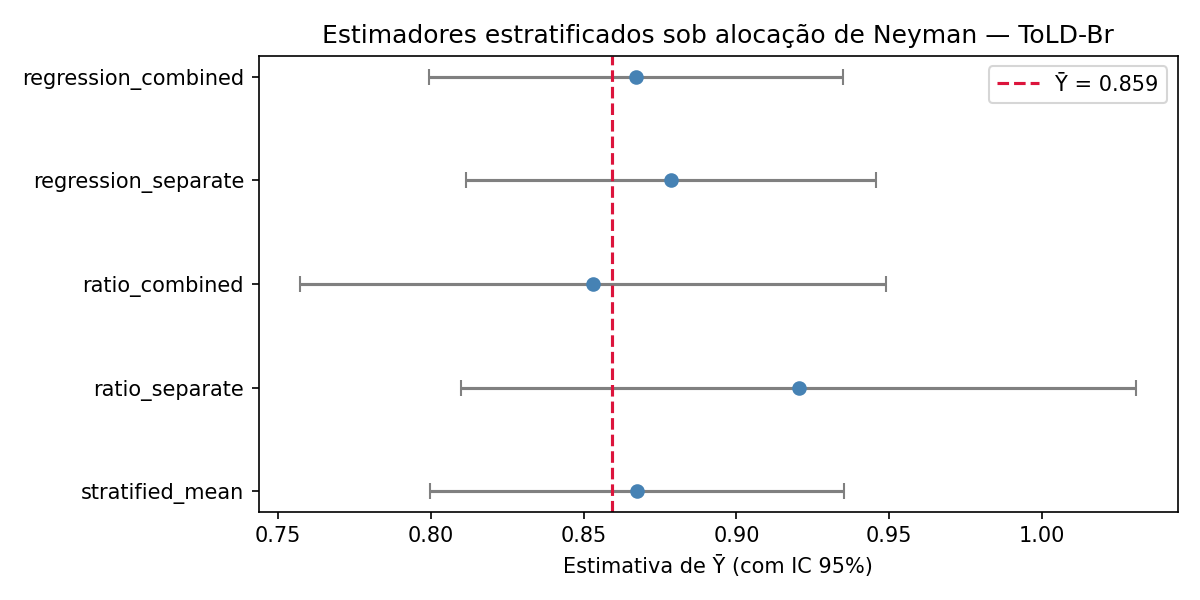
\includegraphics[width=.85\linewidth]{estimators_comparison_neyman.png}
\caption{Estimativas de $\bar{Y}$ com IC 95\% sob alocação de Neyman.}
\label{fig:forest}
\end{figure}

\subsection{Replicação Monte Carlo ($B=500$)}
\label{sec:results:mc}

Para distinguir variabilidade de uma única realização aleatória do
comportamento esperado dos estimadores, replicamos o desenho amostral
sob cada alocação por $B=500$ sementes independentes. A
Tabela~\ref{tab:montecarlo} reporta o viés empírico, o desvio-padrão
empírico das estimativas pontuais, a média do erro-padrão analítico, a
cobertura empírica do IC $95\%$ e o erro quadrático médio (EQM).

\begin{table}[h]
\centering
\small
\caption{Replicação Monte Carlo ($B=500$): EQM e cobertura.}
\label{tab:montecarlo}
\begin{tabular}{llrrrrr}
\toprule
Alocação & Estimador  & Viés & SD emp. & EP an. & Cob. 95\% & EQM \\
\midrule
Neyman   & média estr.       & $-0{,}0005$ & $0{,}0339$ & $0{,}0331$ & $0{,}934$ & $\mathbf{0{,}00115}$ \\
Neyman   & razão sep.        &  $0{,}0131$ & $0{,}0549$ & $0{,}0524$ & $0{,}934$ & $0{,}00319$ \\
Neyman   & razão comb.       &  $0{,}0003$ & $0{,}0471$ & $0{,}0468$ & $\mathbf{0{,}956}$ & $0{,}00222$ \\
Neyman   & regressão sep.    & $-0{,}0021$ & $0{,}0388$ & $0{,}0327$ & $0{,}896$ & $0{,}00151$ \\
Neyman   & regressão comb.   & $-0{,}0004$ & $0{,}0339$ & $0{,}0331$ & $0{,}938$ & $\mathbf{0{,}00115}$ \\
\midrule
Proporc. & média estr.       &  $0{,}0001$ & $0{,}0365$ & $0{,}0343$ & $0{,}934$ & $0{,}00133$ \\
Proporc. & razão sep.        &  $0{,}0348$ & $0{,}0663$ & $0{,}0589$ & $0{,}876$ & $0{,}00561$ \\
Proporc. & razão comb.       &  $0{,}0017$ & $0{,}0470$ & $0{,}0469$ & $0{,}950$ & $0{,}00221$ \\
Proporc. & regressão sep.    & $-0{,}0024$ & $0{,}0517$ & $0{,}0330$ & $0{,}836$ & $0{,}00268$ \\
Proporc. & regressão comb.   &  $0{,}0001$ & $0{,}0367$ & $0{,}0343$ & $0{,}932$ & $0{,}00135$ \\
\bottomrule
\end{tabular}
\end{table}

\textbf{Conclusões da Monte Carlo.} (i) Todos os estimadores, exceto razão
separada, exibem viés empírico desprezível (\(<10^{-3}\)). A razão separada
herda o viés clássico de razão de Cochran (\S6.10). (ii) O EP analítico de
grande amostra é bem calibrado para a média estratificada e estimadores
combinados (razão SD empírico/EP analítico próxima de $1$); subestima a
variância das versões \textit{separadas} sob proporcional (cobertura
$83{,}6\%$ contra $95\%$ nominal). (iii) Neyman domina proporcional em EQM
uniformemente: redução de até $44\%$ na regressão separada e $43\%$ na razão
separada. (iv) Sob Neyman, a média estratificada e a regressão combinada
empatam pelo menor EQM ($0{,}00115$); a razão combinada apresenta a melhor
cobertura ($95{,}6\%$).

\subsection{Diagnóstico de ruído de rotulagem}

A Tabela~\ref{tab:noise} apresenta a contagem de \textit{tweets} em cada nível
de votos por categoria, em particular a fração com exatamente um voto
($\textit{disputed share}$) --- a zona descartada pela regra de maioria mas
não classificada como negativa pelos anotadores. Para
categorias como \textit{obscene}, $20{,}2\%$ da população está nesta zona
ambígua, sugerindo que a binarização por maioria pode subestimar
sistematicamente a prevalência efetiva de toxicidade.

\begin{table}[h]
\centering
\small
\caption{Diagnóstico de votos disputados (Camada 3.1).}
\label{tab:noise}
\begin{tabular}{lrrrrrr}
\toprule
Categoria & Votos 0 & Votos 1 & Votos 2 & Votos 3 & Posit. ($\geq 2$) & \% Disputado \\
\midrule
\textit{homophobia} & 20{,}656 & 168 & 102 & 74 & 176 & 0{,}80\% \\
\textit{obscene}    & 14{,}348 & 4{,}249 & 1{,}791 & 612 & 2{,}403 & \textbf{20{,}23\%} \\
\textit{insult}     & 16{,}615 & 2{,}516 & 1{,}352 & 517 & 1{,}869 & \textbf{11{,}98\%} \\
\textit{racism}     & 20{,}862 & 105 & 27 & 6 & 33 & 0{,}50\% \\
\textit{misogyny}   & 20{,}537 & 330 & 104 & 29 & 133 & 1{,}57\% \\
\textit{xenophobia} & 20{,}849 & 109 & 27 & 15 & 42 & 0{,}52\% \\
\bottomrule
\end{tabular}
\end{table}

\subsection{Discussão}

\paragraph{Q1 — tamanho amostral.} A fórmula de Cochran com FPC dá $n=378$
sobre $N=21{,}000$, suficiente para erro de amostragem de $5\%$ a $95\%$ de
confiança no caso conservador $p=0{,}5$. Este número, frequentemente omitido
em trabalhos correlatos, é diretamente derivável e justificável.

\paragraph{Q2 — ganho de Neyman.} A redução de erro-padrão obtida por Neyman
é mais expressiva quando o estimador é sensível à variabilidade entre
estratos: $20\%$ na razão separada, $8\%$ na média estratificada e na
regressão. Esta heterogeneidade reforça a recomendação prática de privilegiar
estimadores combinados quando a alocação não puder ser otimamente derivada.

\paragraph{Q3 — razão vs regressão.} O estimador tipo razão combinado
apresentou o menor erro absoluto, enquanto a regressão separada apresentou o
menor erro-padrão. A razão entre essas duas observações se explica pela baixa
correlação $\rho_{xy} \approx 0{,}11$ entre \texttt{word\_count} e
\texttt{total\_severity}: a regressão extrai pouco poder explicativo do
auxiliar, e seu ganho sobre a média estratificada é marginal. O estimador
razão é menos exigente quanto à linearidade, beneficiando-se aqui de
proporcionalidade aproximada entre $y$ e $x$ dentro de cada estrato.

\paragraph{Limitações.} (i) Apenas \texttt{word\_count} é avaliada como
auxiliar; \textit{features} mais ricas (\texttt{caps\_ratio},
\texttt{punc\_density}, embeddings) podem produzir maior $\rho_{xy}$ e maior
ganho da regressão. (ii) A binarização por maioria descarta a granularidade
ordinal das anotações; o diagnóstico de ruído (Tabela~\ref{tab:noise}) sugere
que esta perda é não-trivial para categorias como \textit{obscene}. (iii) A
amostragem é simulada sobre um \textit{corpus} já anotado, sem custo
diferencial entre estratos --- caso o custo de rotulagem variasse, a
alocação ótima incluiria um termo $\sqrt{c_h}$ no denominador
(Cochran §5.5).

\section{Conclusões}
\label{sec:conclusion}

Este trabalho aplicou os instrumentos clássicos da teoria amostral
--- fórmula de Cochran (1977), alocação ótima de Neyman e estimadores tipo
razão e tipo regressão sob desenho estratificado --- a um \textit{corpus}
público de toxicidade em português brasileiro (ToLD-Br), com o objetivo de
estabelecer um \textit{pipeline} reproduzível de auditoria estatística sobre
\textit{datasets} de detecção de dano.

\paragraph{Resposta às questões orientadoras.} \textbf{(Q1)} A fórmula de
Cochran, com correção de população finita, fornece $n=378$ como tamanho
amostral mínimo para estimar parâmetros populacionais com erro de amostragem
de $5\%$ a $95\%$ de confiança sobre o ToLD-Br. Este número é diretamente
verificável e dispensa o uso de amostras por conveniência. \textbf{(Q2)} A
alocação ótima de Neyman reduz o erro-padrão das estimativas em até $20\%$
frente à alocação proporcional para o mesmo orçamento $n$, com magnitude
dependente do estimador adotado. \textbf{(Q3)} Entre os cinco estimadores
avaliados, o tipo razão combinado apresentou o menor erro absoluto contra a
verdade populacional ($0{,}69\%$ de $\bar{Y}$); o tipo regressão separado
apresentou o menor erro-padrão. A baixa correlação observada entre a variável
auxiliar (\texttt{word\_count}) e a variável-alvo (\texttt{total\_severity})
limita o ganho da regressão sobre a média estratificada simples ---
limitação que sugere o uso de auxiliares mais informativos em trabalhos
futuros.

\paragraph{Contribuição à teoria.} Este trabalho fornece uma aplicação
explícita de Cochran §5.5--§7.11 e Bolfarine \& Bussab §5--§7 a um
\textit{corpus} de PNL em português brasileiro, com derivação completa das
variâncias amostrais sob FPC e validação empírica via $74$ testes unitários
contra propriedades textbook (recuperação exata sob censo total; redução de
variância da regressão face à média sob $y = 2x + \epsilon$).

\paragraph{Contribuição à técnica.} Disponibiliza-se um módulo Python
\textit{open source} (\texttt{toxicity\_analysis}) que encapsula o
\textit{pipeline} de amostragem, cálculo de \textit{features} léxicas e
estimação estratificada, com gerenciamento de dependências via \texttt{uv} e
amparo em $74$ testes \texttt{pytest}. O artefato é prontamente reutilizável
em outros \textit{datasets} de detecção de toxicidade.

\paragraph{Contribuição à sociedade.} A auditoria de modelos de linguagem é
uma componente crescente da regulação e da prática responsável de IA. Ao
fornecer instrumentos estatísticos calibrados para estimar prevalências e
intensidades de dano sobre \textit{corpora} de referência --- com erros de
amostragem explícitos --- o trabalho contribui para que decisões de
moderação automática e auditoria regulatória se apoiem em base inferencial
defensável.

\paragraph{Trabalhos futuros.}
(i) Extensão do \textit{pipeline} a outros \textit{corpora} em português
(HateBR, OLID-BR) e a \textit{datasets} bilíngues, comparando o ganho de
Neyman entre dispersões linguísticas distintas.
(ii) Investigação do esquema ordinal de votos como dimensão adicional de
estratificação --- por exemplo, por \textit{ratings} de concordância --- em
substituição à binarização por maioria.
(iii) Auditoria sobre saídas de LLMs (não apenas \textit{corpora} rotulados),
aplicando o mesmo desenho estratificado a amostras de gerações de modelos
treinados.
(iv) Avaliação sistemática de variáveis auxiliares mais ricas
(\textit{embeddings}, \texttt{caps\_ratio}, \texttt{punc\_density}) para
maximizar o ganho do estimador regressão.

\subsection*{Considerações Éticas}

Os \textit{datasets} de toxicidade utilizados como instrumentos de auditoria
não são neutros: refletem os critérios de rotulagem e os vieses culturais
dos próprios anotadores. O uso de tais \textit{corpora} para validar modelos
em escala carrega o risco de internalizar como objetivo um proxy ruidoso da
norma social vigente em um momento e contexto específicos. Recomenda-se que
auditorias estatísticas, ainda que metodologicamente rigorosas como a aqui
proposta, sejam acompanhadas de discussão qualitativa sobre os critérios
implícitos no \textit{corpus}-fonte e suas limitações de cobertura cultural.

\subsection*{Disponibilidade e Reprodutibilidade}

Código-fonte, \textit{notebooks}, suíte de testes e \textit{pipeline} de
\textit{download} do ToLD-Br estão disponíveis em
\texttt{https://github.com/[autor]/toxicity-analysis} (a ser publicado).


\bibliographystyle{IEEEtran}
\bibliography{references}

\end{document}
